%!TEX root = ../GLM_Becerra_Lopez.tex

\section{Modelos estadísticos}
\label{sec:modelos}

El objetivo es obtener estimaciones del precio de las casas a partir del tamaño en pies cuadrados. Para probar la capacidad predictiva, se dividieron los datos en dos: un conjunto de entrenamiento con el 90\% de los datos, y un conjunto de prueba con el 10\% restante. Para tener información de todos los códigos postales, se hizo un muestreo estratificado, tomando el 90\% de observaciones de cada código postal para el conjunto de entrenamiento. En el conjunto de entrenamiento quedaron $22,769$ observaciones y en el de prueba $2,530$.	

Se ajustaron tres modelos lineales a los datos: un modelo de unidades iguales, un modelo de unidades independientes, y un modelo jerárquico. El modelo de unidades iguales asume que todas las realizaciones provienen de la misma distribución; mientras que el de unidades independientes asume que los precios varían de acuerdo a diferentes sectores (en este caso son los códigos postales); y finalmente, el modelo jerárquico es un compromiso entre ambos modelos que toma fuerza de los demás sectores, esto es particularmente útil cuando hay sectores con pocas observaciones.

\subsection{Modelo de unidades iguales}

El modelo de unidades iguales es simplemente un modelo de regresión lineal con un parámetro fijo para el intercepto y un parámetro fijo para cada uno de los regresores. Sean $y_i$ el logaritmo del precio de la casa $i$ y $x_i$ el logaritmo del número de pies cuadrados en la casa $i$, para $i \in \left\{1, \hdots, n \right\}$, con $n = 22,769$. El modelo de unidades independientes es $y_i \sim \mathrm{N}(\alpha + \beta x_i, \tau_y)$, con distribuciones previas $\alpha \sim \mathrm{N}(0, 0.001)$, $\beta \sim \mathrm{N}(0, 0.001)$ y $\tau_y \sim \mathrm{Ga}(0.001, 0.001)$. %$\alpha \sim \mathrm{N}(\alpha_0, \tau_{\alpha})$, $\beta \sim \mathrm{N}(\beta_0, \tau_{\beta})$ y $\tau_y \sim \mathrm{Ga}(a, b)$

De antemano se tiene conocimiento como para pensar que este modelo no es el más adecuado para los datos, pues se vio en el análisis exploratorio de datos que los precios varían por código postal, por lo que no es muy sensato suponer que no existen relaciones entre las observaciones.

De hecho, en la figura \ref{fig:comp_pooling_resids} se puede ver este efecto. En la figura se muestran los residuales del modelo en el eje $y$, y en el eje $x$ se muestra el índice de la observación, donde las observaciones están ordenadas de acuerdo a código postal. Es evidente un patrón, que viene de la correlación entre las observaciones que existe dentro de cada código postal.

\begin{figure}[H]
    \centering
    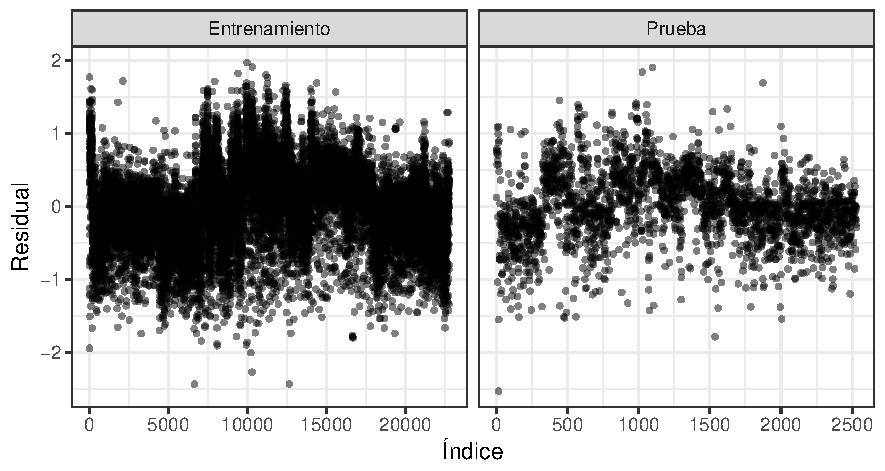
\includegraphics[width=0.9\textwidth]{images/comp_pooling_resids.pdf}
    \caption{Residuales de modelo de unidades iguales}
    \label{fig:comp_pooling_resids}
\end{figure}

En la figura \ref{fig:comp_pooling_obs_vs_pred} se puede ver para cada observación el valor observado contra el valor ajustado. Se aprecia una varianza considerablemente grande y que además en los valores pequeños, el modelo tiende a sobreestimar, mientras que en valores grandes pasa lo contrario.

\begin{figure}[H]
    \centering
    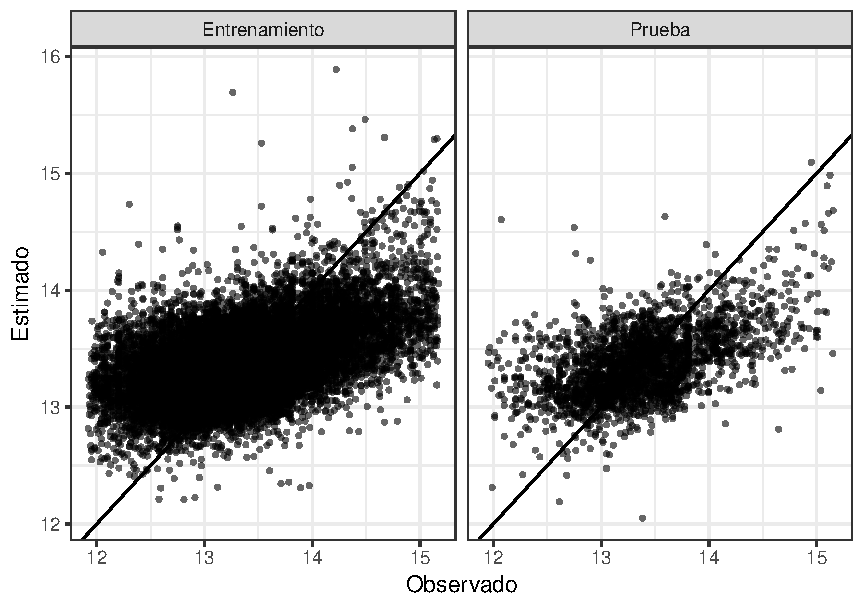
\includegraphics[width=0.9\textwidth]{images/comp_pooling_obs_vs_pred.pdf}
    \caption{Ajustado contra observado en modelo de unidades iguales}
    \label{fig:comp_pooling_obs_vs_pred}
\end{figure}

\subsection{Modelo de unidades independientes}

Este es un modelo de interceptos y pendientes cambiantes de acuerdo al código postal, es decir, es de la forma $y_i \sim \mathrm{N}(\alpha_{j[i]} + \beta_{j[i]}, \tau_y)$, donde $j[i]$ se refiere al código postal correspondiente a la $i$-ésima observación. Las distribuciones previas son $\alpha[j] \sim \mathrm{N}(0, 0.001)$, $\beta[j] \sim \mathrm{N}(0, 0.001)$ y $\tau_y \sim \mathrm{Ga}(0.001, 0.001)$, para $j = 1, \hdots, J$, con $J = 154$ el número de códigos postales en la ciudad.

\begin{figure}[H]
    \centering
    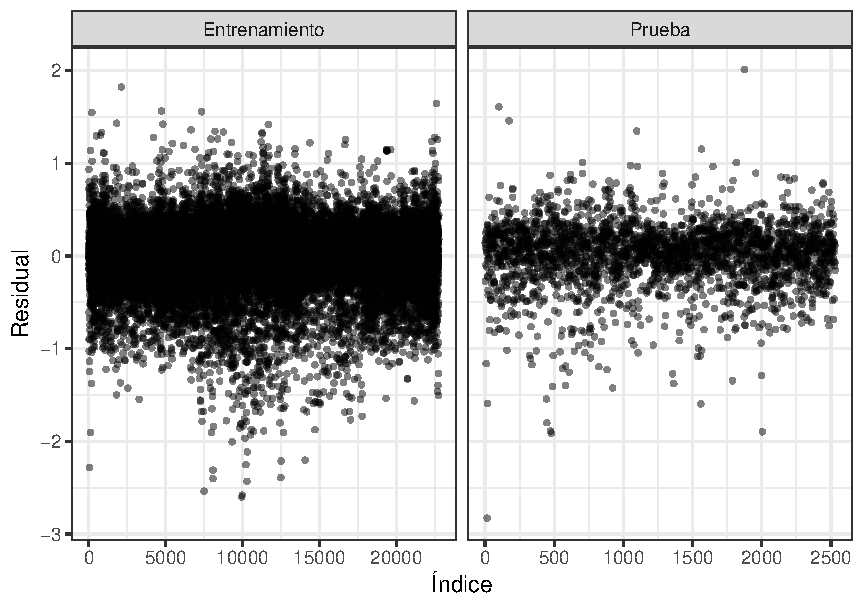
\includegraphics[width=0.9\textwidth]{images/no_pooling_resids.pdf}
    \caption{Residuales de modelo de unidades independientes}
    \label{fig:no_pooling_resids}
\end{figure}

\begin{figure}[H]
    \centering
    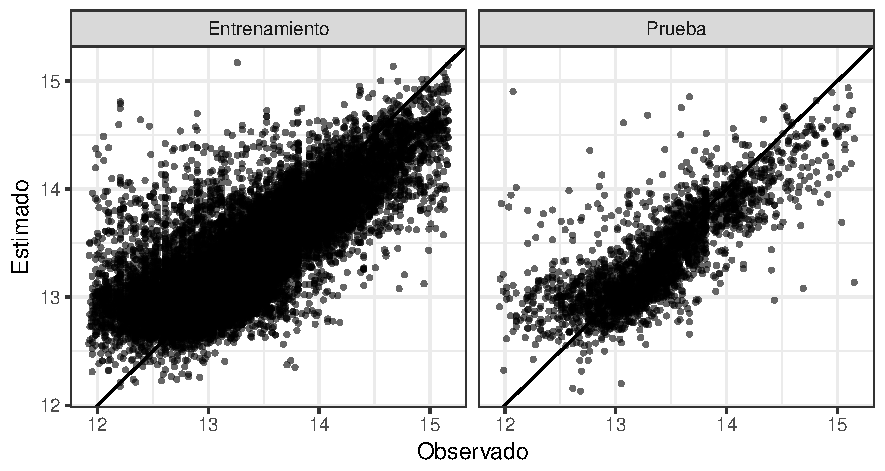
\includegraphics[width=0.9\textwidth]{images/no_pooling_obs_vs_pred.pdf}
    \caption{Valor ajustado contra observado en modelo de unidades independientes}
    \label{fig:no_pooling_obs_vs_pred}
\end{figure}

\begin{figure}[H]
    \centering
    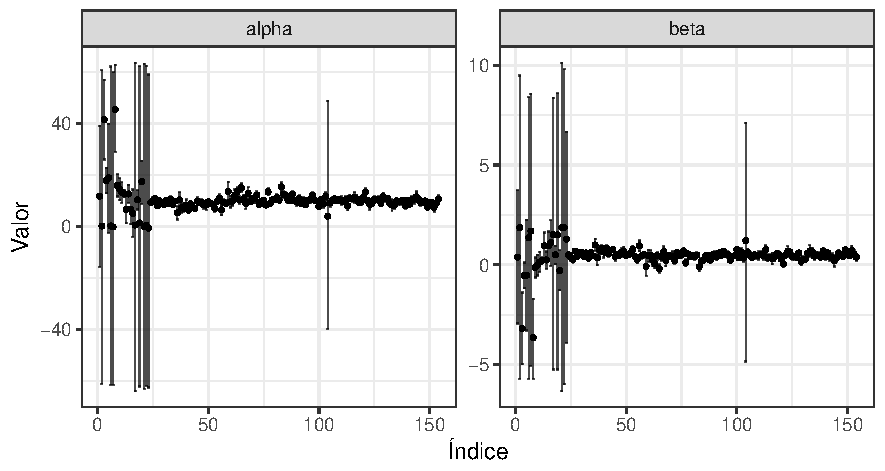
\includegraphics[width=0.9\textwidth]{images/no_pooling_param_values.pdf}
    \caption{Valor e intervalos de probabilidad de parámetros de modelo de unidades independientes}
    \label{fig:no_pooling_param_values}
\end{figure}


\subsection{Modelo multinivel}



\begin{figure}[H]
    \centering
    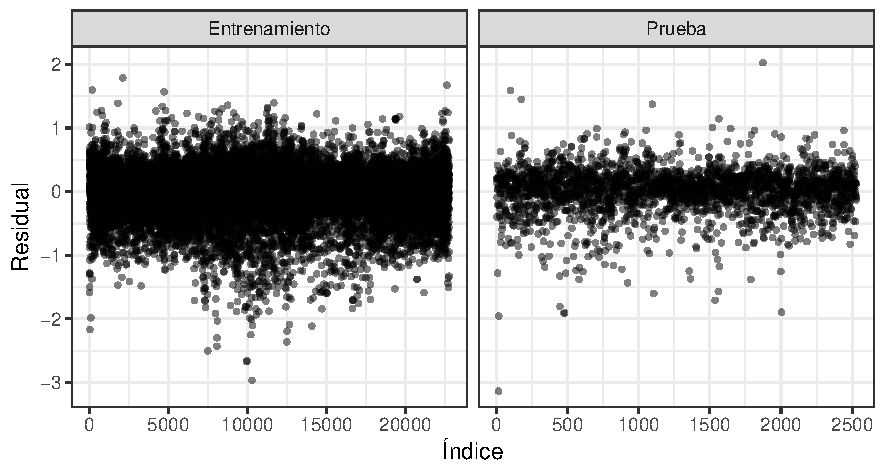
\includegraphics[width=0.9\textwidth]{images/three_levels_resids.pdf}
    \caption{Residuales de modelo multinivel}
    \label{fig:three_levels_resids}
\end{figure}

\begin{figure}[H]
    \centering
    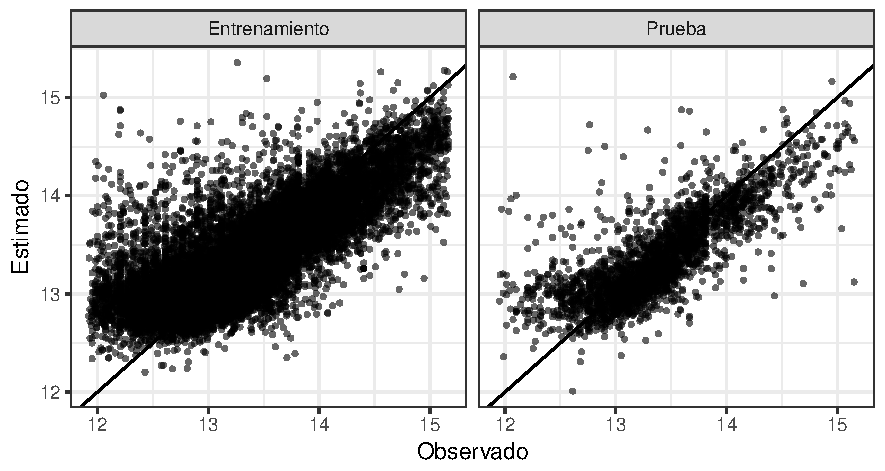
\includegraphics[width=0.9\textwidth]{images/three_levels_obs_vs_pred.pdf}
    \caption{Valor ajustado contra observado en modelo multinivel}
    \label{fig:three_levels_obs_vs_pred}
\end{figure}

\begin{figure}[H]
    \centering
    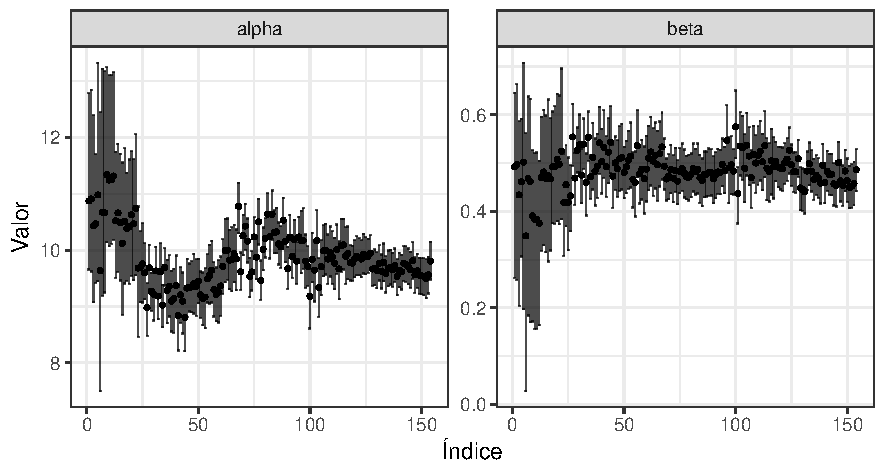
\includegraphics[width=0.9\textwidth]{images/three_levels_param_values.pdf}
    \caption{Valor e intervalos de probabilidad de parámetros de modelo multinivel}
    \label{fig:three_levels_param_values}
\end{figure}
